\section{Results}
\label{sec:results}

\para{Main judged scores.} \Tabref{tab:main_scores} summarizes all judged and automatic metrics by condition. The strongest grounded condition by overall quality is \litcompare, with mean overall 4.00 compared with 3.92 for \ungrounded. This is a small absolute gain of 0.08 points on a 1--5 scale. The \ungrounded baseline remains strongest on the \nfprod, with a mean of 14.67 compared with 14.33 for \litcompare and 14.00 or lower for the other grounded conditions.

\begin{table*}[t]
    \centering
    \resizebox{\textwidth}{!}{%
    \begin{tabular}{@{}lrrrrrrrr@{}}
        \toprule
        \textbf{Condition} & \textbf{$n$} & \textbf{Novelty} & \textbf{Feas.} & \textbf{Spec.} & \textbf{Ground.} & \textbf{Overall} & \textbf{Nov.$\times$Feas.} & \textbf{Prior Overlap} \\
        \midrule
        \ungrounded & 12 & {\bf 3.75} & 3.92 & {\bf 3.92} & 3.92 & 3.92 & {\bf 14.67} & {\bf 0.043} \\
        \deduction & 12 & 3.50 & 3.83 & 3.67 & 4.00 & 3.75 & 13.33 & 0.077 \\
        \induction & 12 & 3.42 & {\bf 4.00} & 3.75 & 4.00 & 3.75 & 13.67 & 0.092 \\
        \proposal & 12 & 3.58 & 3.92 & {\bf 3.92} & 4.00 & 3.92 & 14.00 & 0.073 \\
        \outcome & 12 & 3.50 & {\bf 4.00} & 3.75 & 4.00 & 3.83 & 14.00 & 0.059 \\
        \smallexperiment & 12 & 3.33 & {\bf 4.00} & 3.58 & 4.00 & 3.58 & 13.33 & 0.065 \\
        \litcompare & 12 & {\bf 3.75} & 3.83 & 3.75 & {\bf 4.08} & {\bf 4.00} & 14.33 & 0.106 \\
        \bottomrule
    \end{tabular}
    }
    \caption{Mean scores by condition. Judged scores are on a 1--5 scale. Higher is better except prior-work overlap, where lower means less lexical reuse from prior-work titles. Best values are in \textbf{bold}.}
    \label{tab:main_scores}
\end{table*}


\Figref{fig:condition_scores} shows the judged score distributions by condition. The main visual pattern is compression: most scores fall between 3 and 4, with limited separation among prompt variants. This ceiling makes large gains unlikely and makes paired tests important.

\begin{figure}[t]
    \centering
    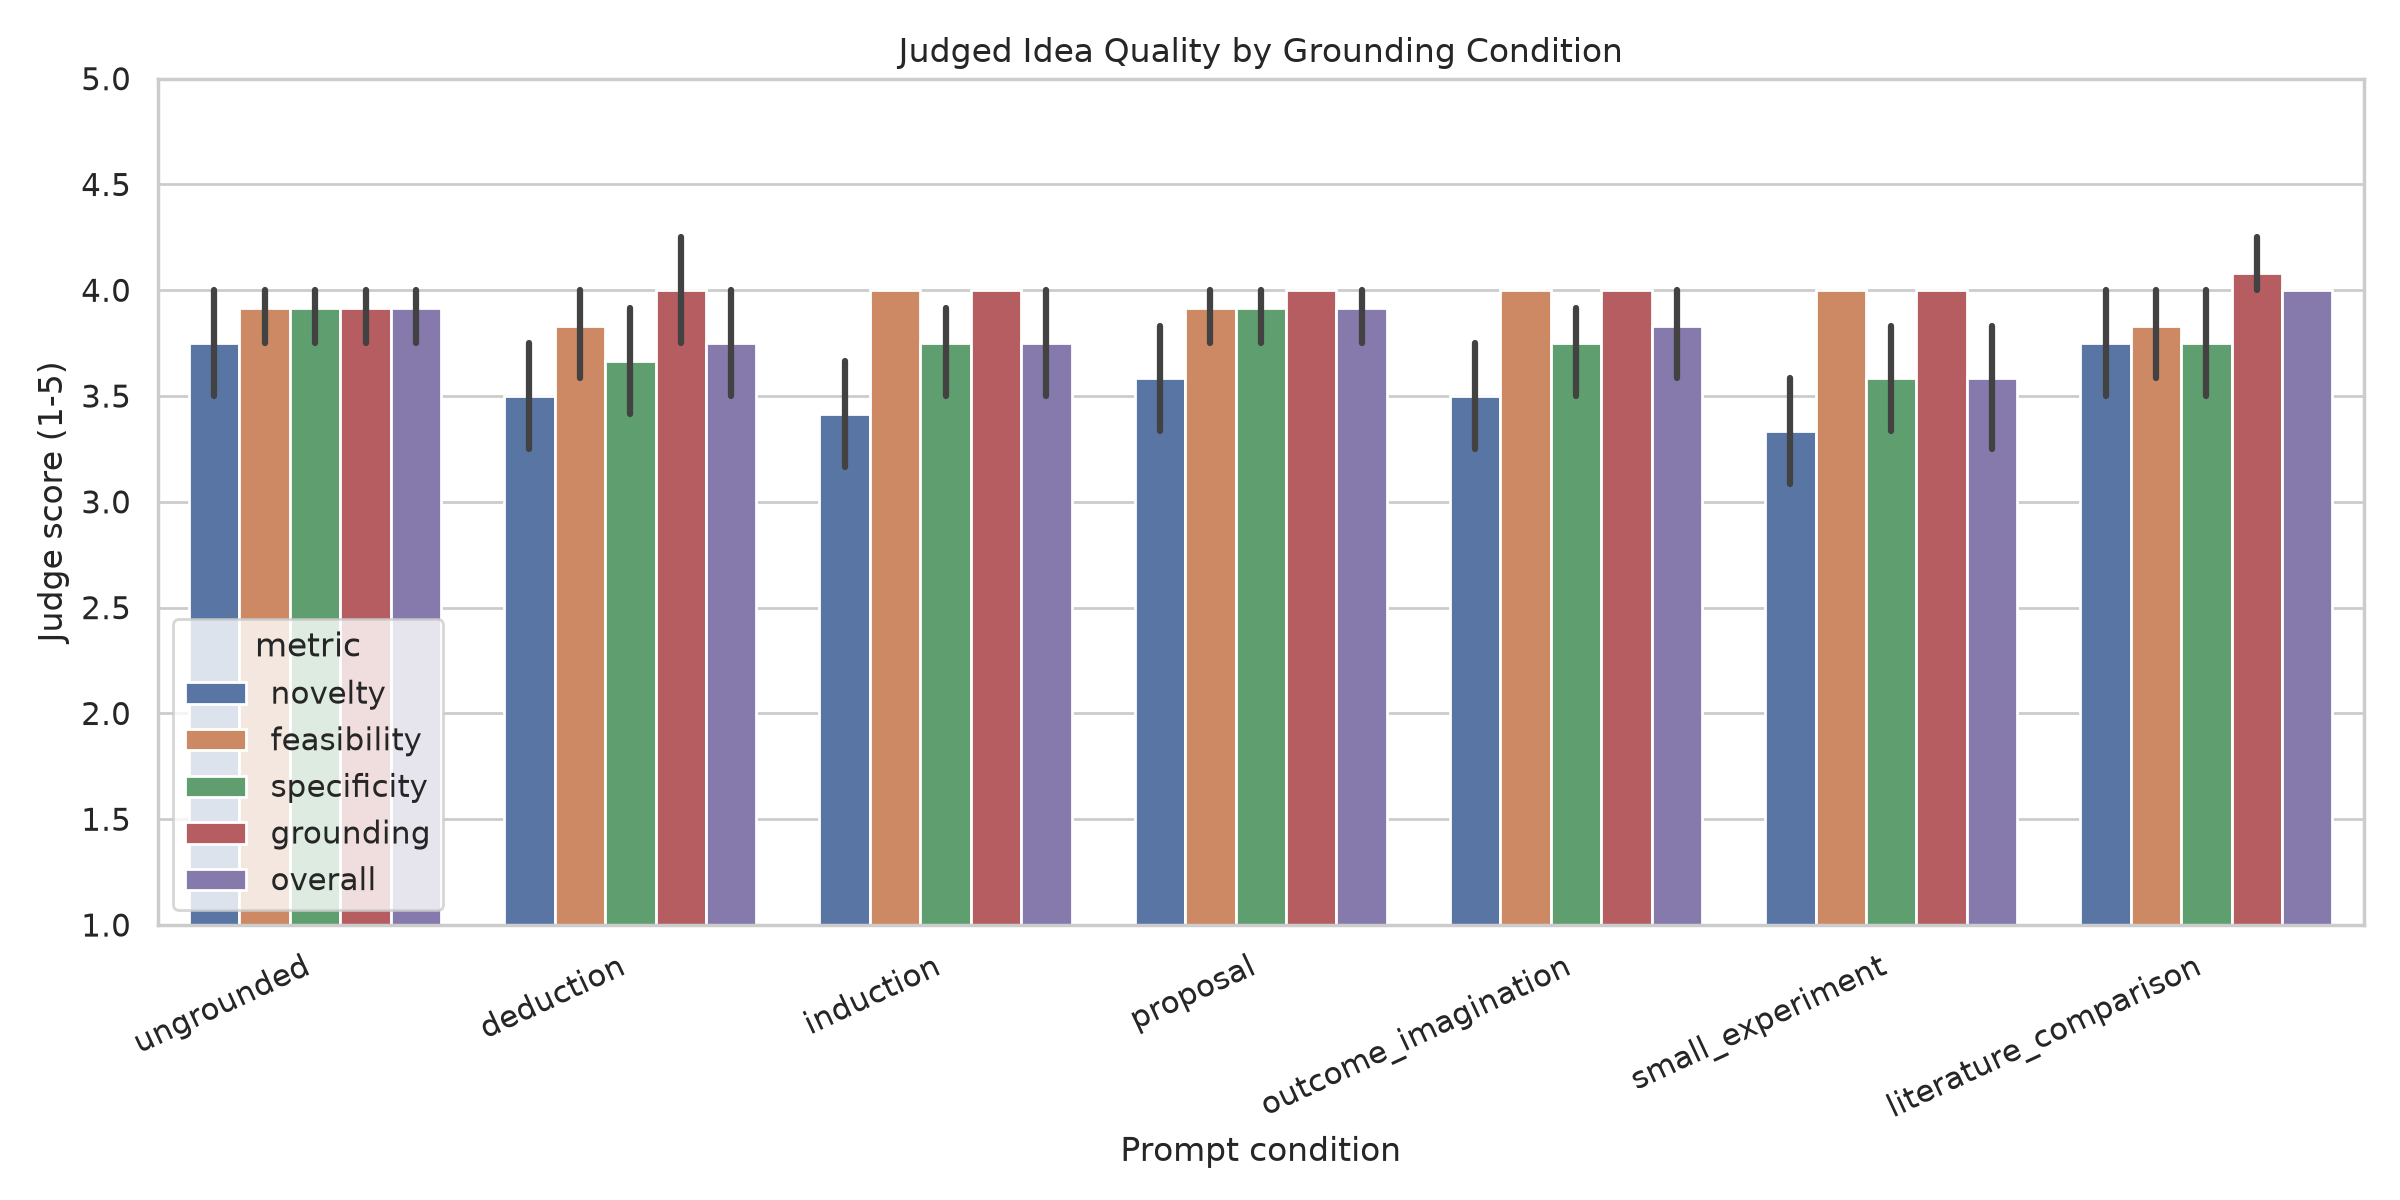
\includegraphics[width=0.95\linewidth]{figures/condition_scores.png}
    \caption{Judged idea quality by prompt condition. The grounded prompt variants do not separate cleanly from the \ungrounded baseline on novelty, feasibility, specificity, grounding, or overall quality.}
    \label{fig:condition_scores}
\end{figure}

\para{Omnibus tests.} \Tabref{tab:omnibus} reports Friedman tests across all seven conditions. No judged quality metric shows a significant condition effect. Overall quality has $p=0.157$, quality mean has $p=0.208$, and \nfprod has $p=0.572$. Grounding score itself also does not significantly differ across conditions ($p=0.701$), despite grounded prompts being more explicit about prior work.

\begin{table}[t]
    \centering
    \resizebox{0.92\textwidth}{!}{%
    \begin{tabular}{@{}lrr@{}}
        \toprule
        \textbf{Metric} & \textbf{Friedman statistic} & \textbf{$p$-value} \\
        \midrule
        Novelty & 8.60 & 0.197 \\
        Feasibility & 7.29 & 0.295 \\
        Specificity & 6.59 & 0.361 \\
        Grounding & 3.82 & 0.701 \\
        Overall & 9.32 & 0.157 \\
        Quality mean & 8.44 & 0.208 \\
        Novelty--feasibility product & 4.78 & 0.572 \\
        Prior-work overlap & {\bf 53.21} & {\bf $1.06\times10^{-9}$} \\
        \bottomrule
    \end{tabular}
    }
    \caption{Omnibus paired tests across all seven conditions and 12 matched contexts. Only prior-work overlap shows a significant condition effect.}
    \label{tab:omnibus}
\end{table}


\para{Prior-work overlap changes sharply.} The one strong condition effect is prior-work overlap. The Friedman statistic is 53.21 with $p=1.06\times10^{-9}$. Every grounded condition has higher overlap than \ungrounded after Holm correction. \litcompare has the largest increase over baseline: $+0.063$ in mean overlap, paired Cohen's $d=2.84$, and Holm-adjusted $p=0.0029$. \Figref{fig:overlap_diversity} shows this pattern together with condition diversity.

\begin{figure}[t]
    \centering
    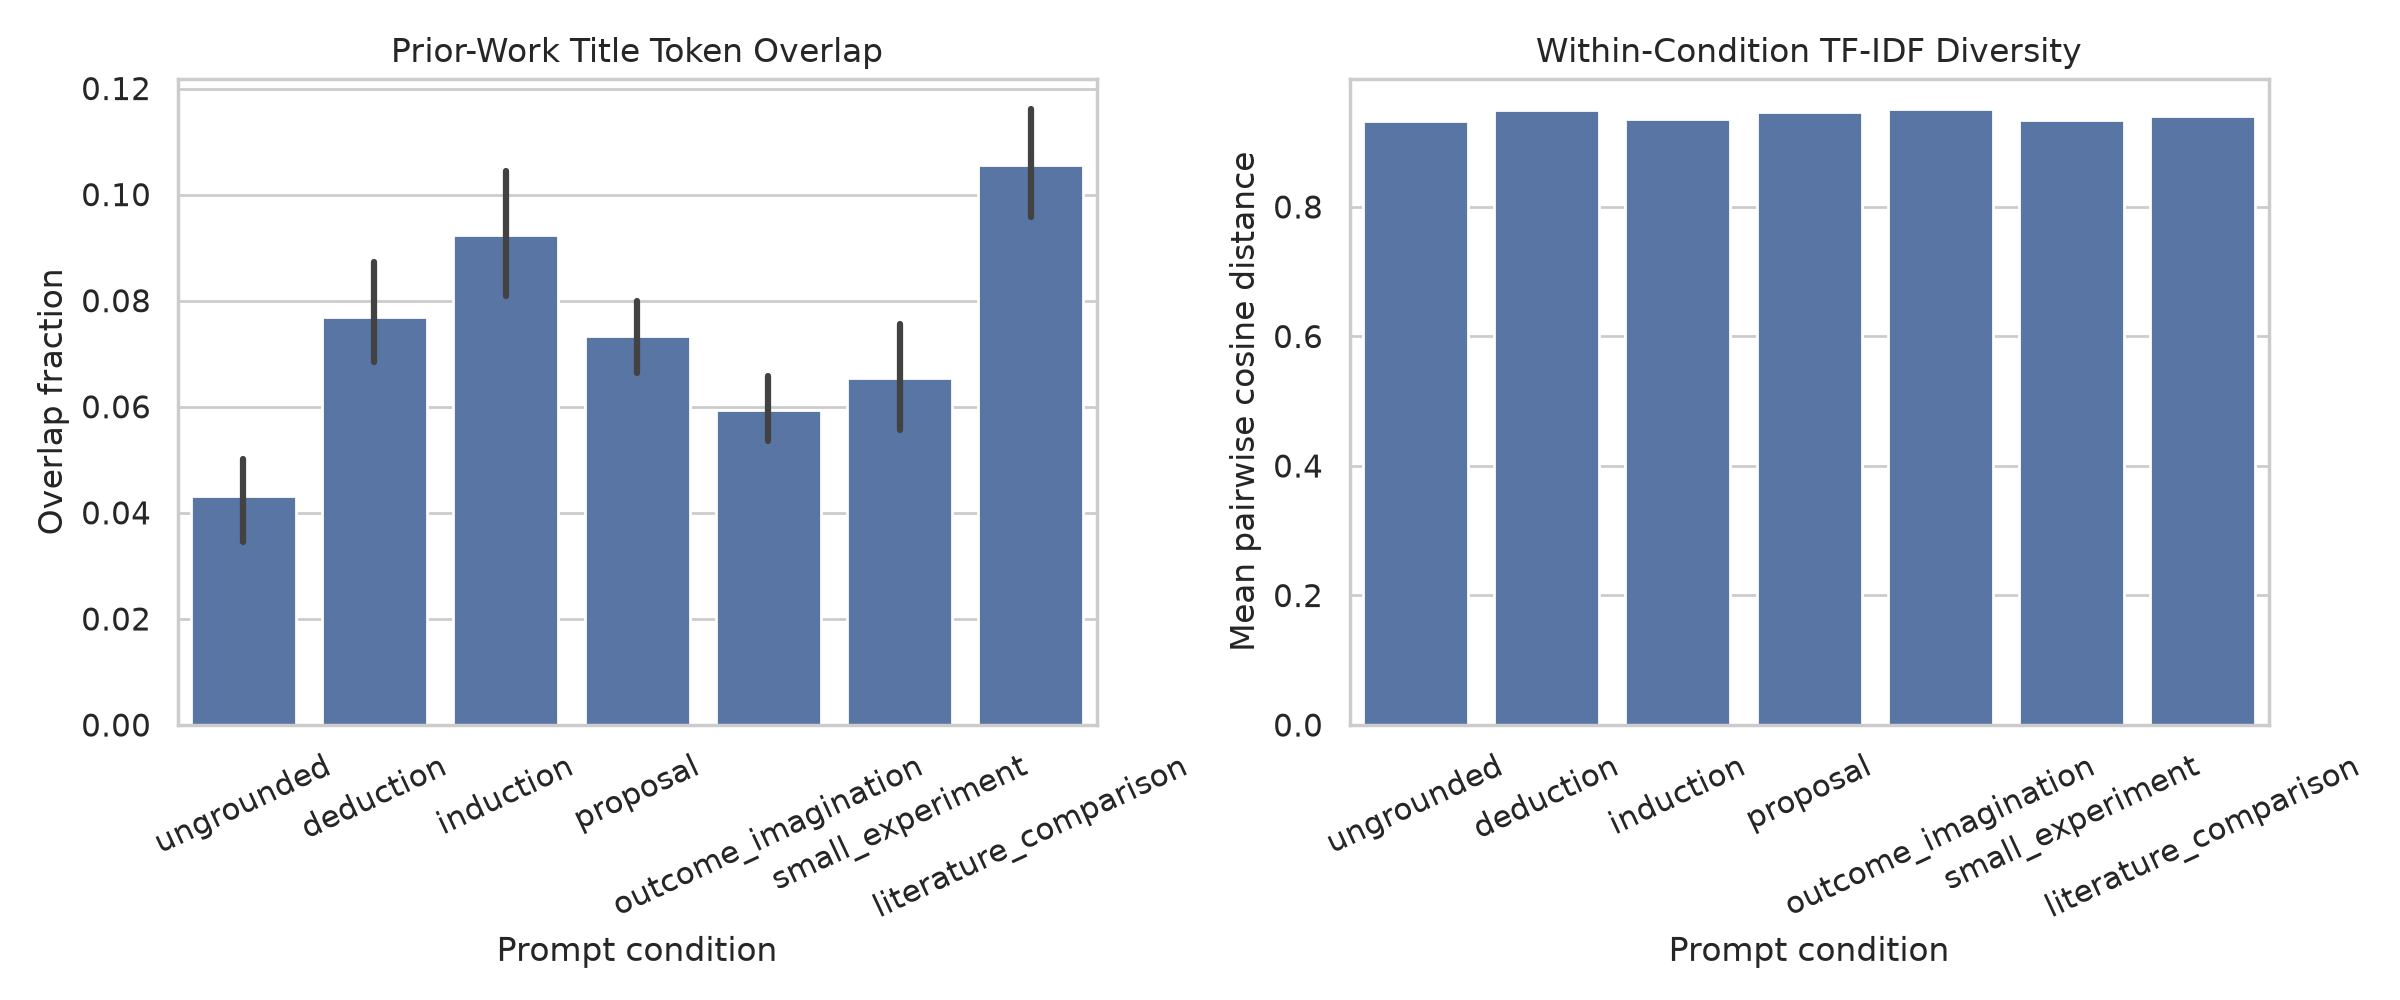
\includegraphics[width=0.95\linewidth]{figures/overlap_diversity.png}
    \caption{Prior-work overlap and within-condition diversity. Grounded prompts consistently increase lexical overlap with prior-work titles, with the largest increase under \litcompare. Diversity remains high across all conditions and does not explain the main judged-score pattern.}
    \label{fig:overlap_diversity}
\end{figure}

\para{Novelty--feasibility tradeoff.} \Figref{fig:nf_product} focuses on the \nfprod. If prompt grounding improved the practical novelty of ideas, we would expect grounded conditions to exceed \ungrounded on this product. Instead, \ungrounded has the highest mean product, 14.67, and all grounded conditions are lower. Pairwise differences versus \ungrounded are not significant after Holm correction, but the direction is important: prompt-level grounding did not improve the intended novelty--feasibility tradeoff.

\begin{figure}[t]
    \centering
    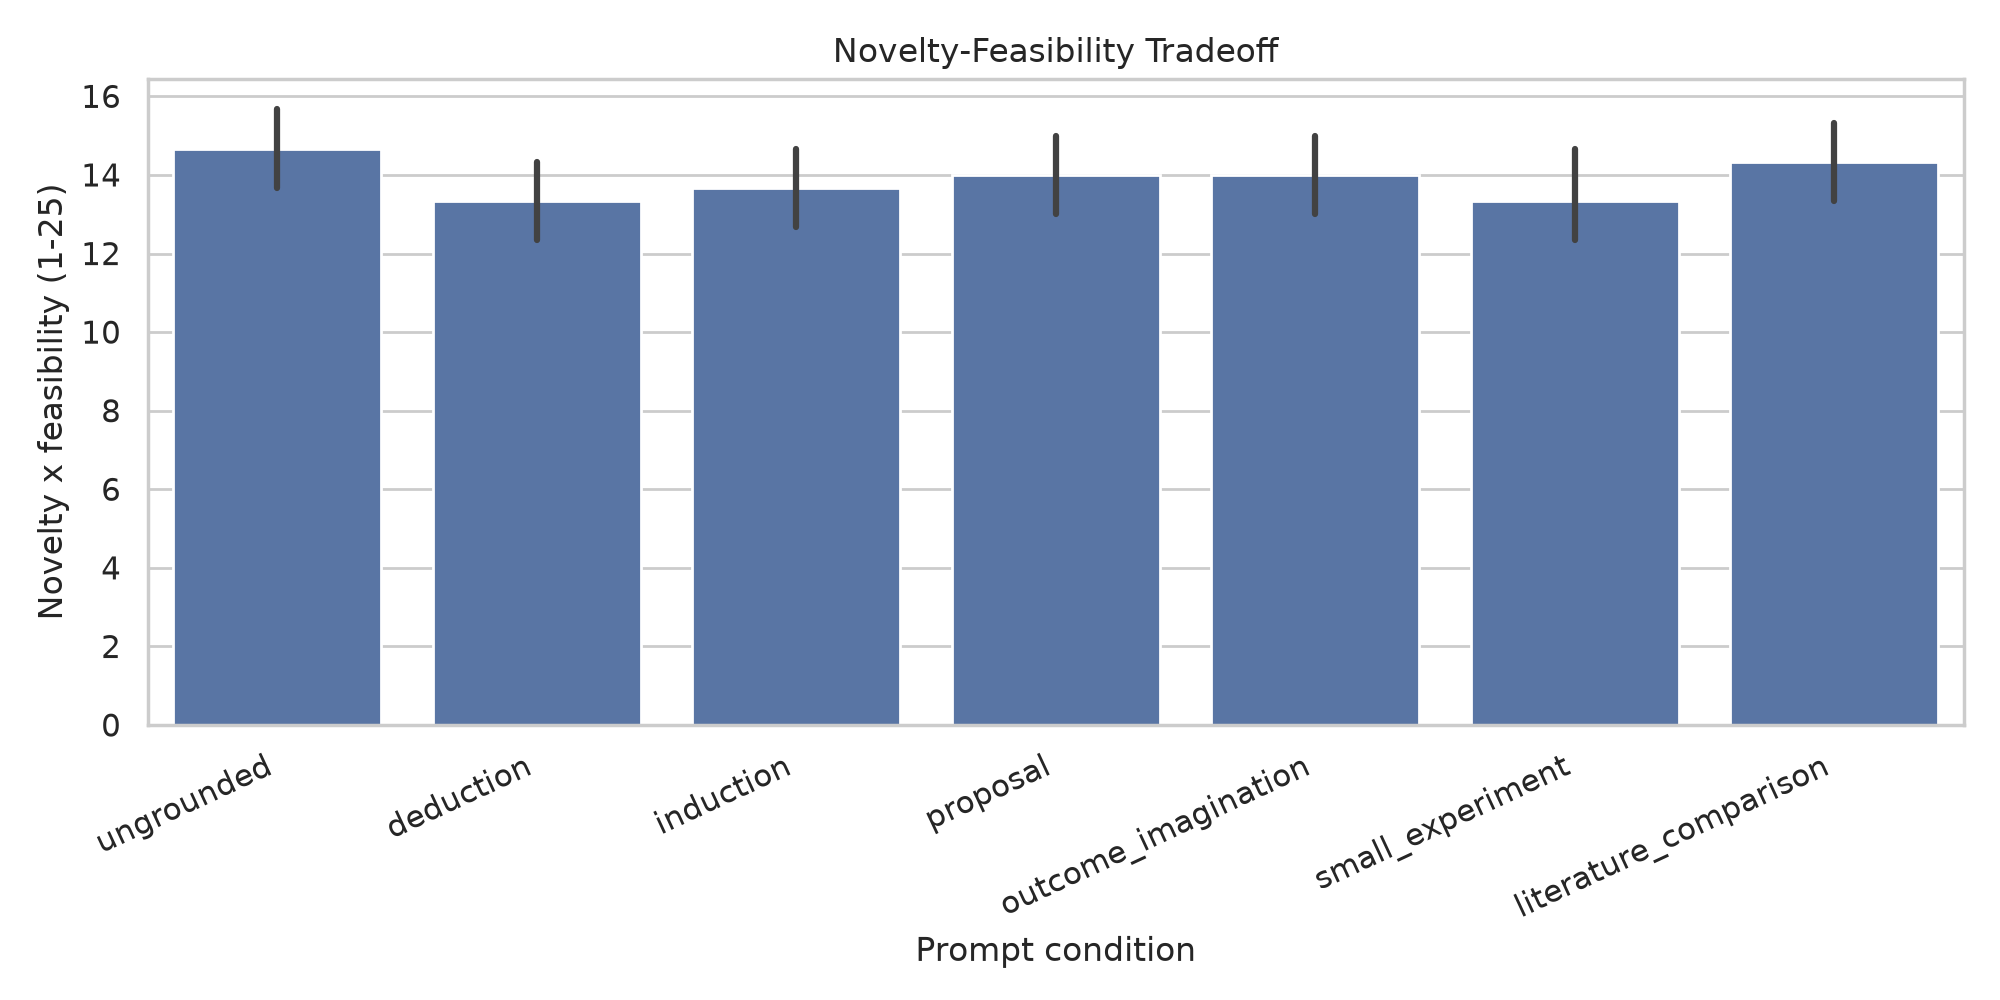
\includegraphics[width=0.82\linewidth]{figures/novelty_feasibility_product.png}
    \caption{Novelty--feasibility product by condition. The \ungrounded baseline has the highest mean product, while grounded conditions do not produce a reliable gain.}
    \label{fig:nf_product}
\end{figure}

\para{Ablation interpretation.} The condition comparison acts as an ablation over grounding operations. \proposal matches \ungrounded on specificity and overall score but does not improve novelty. \outcome keeps feasibility high but does not improve overall quality. \smallexperiment performs worst on novelty, specificity, overall score, quality mean, and \nfprod. The small audit used only title-term frequencies and missing evaluation cues, so this result suggests that empirical grounding must provide meaningful evidence before it can improve idea quality.

\para{Qualitative errors.} Error analysis shows repeated underspecification. Weak ideas often rely on vague mechanisms such as ``adaptive modules,'' ``contrastive heads,'' or unspecified feedback loops. Feasibility scores remain high because the generator can name datasets, baselines, and metrics, but this may reflect proposal fluency rather than true executable strength. \litcompare often writes polished differentiation claims, yet those claims do not consistently raise judged novelty.
